\section{Summary}
\label{sec:conclusion}

This work describes a refined methodology for theoretical wave resource assessment that resolves several outstanding issues with earlier approaches. This work provides a consistent methodology for accounting for wave energy at regional scales, but it can also be applied at the project scale. This consistency at all scales makes it ideally suited for broader adoption by the international community which will in turn make the assessment of market opportunities more comparable and transparent. The methodology proposed in this study demonstrates the importance of including the local resource to accurately assess the total theoretical resources at regional scales. It would benefit the wave energy community if this methodology were incorporated into IEC standards so that there is clarity and consistency on the topic of regional theoretical wave resource assessment, which is the basis for more granular `technical' and 'practical' resource assessments, which are in turn the basis of the wave energy value proposition.

We then apply this methodology to the U.S. EEZ (except for the portion of the EEZ associated with U.S. Pacific Islands Territories), and find that the total U.S. wave energy resource is greater than 3,300 TWh/yr.
This is an increase of ~25\% compared to earlier DOE wave resource assessments, and is due to the combination of extending the resource area to the edge of the EEZ and incorporating the local resource. The `inner shelf' resource (i.e., at 10 nautical-miles from shore) is estimated herein to be 1800 TWh/yr.  As other nations and regions adopt the methodology, these numbers will provide an apples-to-apples comparison of opportunity, which can inform decision making and investment.

\begin{figure}[ht]
  \centering
  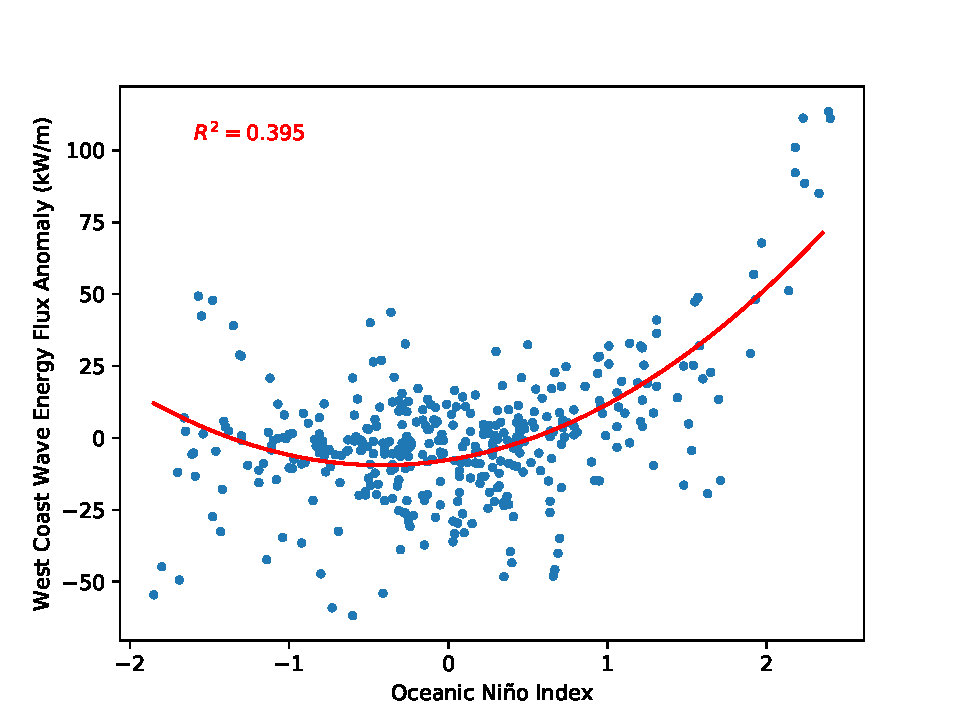
\includegraphics[width=\textwidth]{./fig/ENSO-Comparison.wc.pdf}
  \caption{West Coast wave energy flux anomaly vs. Oceanic Ni\~{n}o Index (ONI). The wave energy flux anomaly (annual cycle removed) is averaged along the EEZ boundary, has had a 5-month running average applied, and lags the ONI signal by 2-months.}
  \label{fig:wc-nino}
\end{figure}

\section{The Future of Wave Energy}
\label{sec:future}

The United States possesses significant wave energy resources (3,300 TWh/yr), especially along its pacific coastlines. However, the technologies for converting this energy into electricity are still at an early stage of development, and several device arch-types are still being explored \citep{babaritOceanWaveEnergy2017}. Narrowing these technologies to a short-list of arch-types that hold the most promise is a challenge. It requires a robust research and development program that maximizes data-collection from device tests, and feeds that data into numerical simulation tools that can be used to refine designs. It also requires a willingness to drop a concept from the candidate pool when fatal flaws are identified.

Undertaking this challenge is worthwhile because success will mean adding a new and sizable resource to our generation mix. These resources may be especially valuable because their variability is distinct compared to other renewables, and they are more predictable than wind and solar. Satellites can observe waves propagating across the ocean, and models can predict where they will go. On inter-annual timescales, ENSO fluctuations are correlated with an increase in the U.S. wave energy resource (Figure \ref{fig:wc-nino}) that is most likely caused by the larger than normal storms that occur in the S. Pacific during El Nino \citep{andersonClimateIndexOptimized2018, yangCharacteristicsVariabilityNearshore2020, ruggieroNationalAssessmentShoreline2013}. Or perhaps—as demand for renewable energy continues to grow—these resources will be valuable simply because they are in the water where land-use and view-shed concerns may be reduced.

%%% Local Variables:
%%% TeX-master: "wave_res"
%%% End:
